\documentclass{article}
\usepackage{tikz, pgfplots}
    \usepgfplotslibrary{external}
    \tikzexternalize
\pgfplotsset{compat=1.18}
\begin{document}

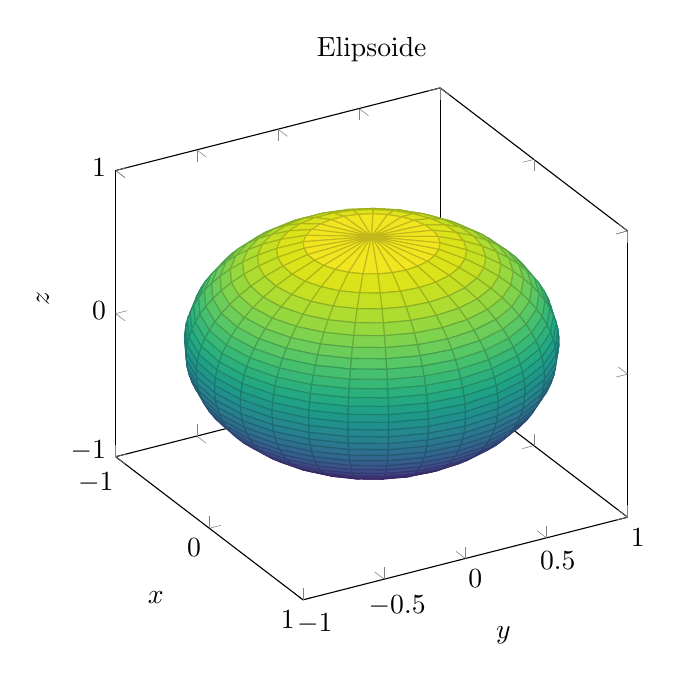
\begin{tikzpicture}
\begin{axis}[
    view={60}{30},
    width=\textwidth/1.5,
    height=\textwidth/1.5,
    xlabel=$x$,
    ylabel=$y$,
    zlabel=$z$,
    z buffer=sort,
    xmin=-1,xmax=1,ymin=-1,ymax=1,zmin=-1,zmax=1,
    title={Elipsoide},
]
\addplot3[
    surf,
    colormap/viridis,
    samples=30,
    samples y=30,
    domain=-1:1,
    y domain=0:2*pi,
    variable=\z,
    variable y=\theta
]
({sqrt(1-\z^2)*cos(deg(\theta))}, {sqrt(1-\z^2)*sin(deg(\theta))}, {0.75*\z});
\end{axis}
\end{tikzpicture}

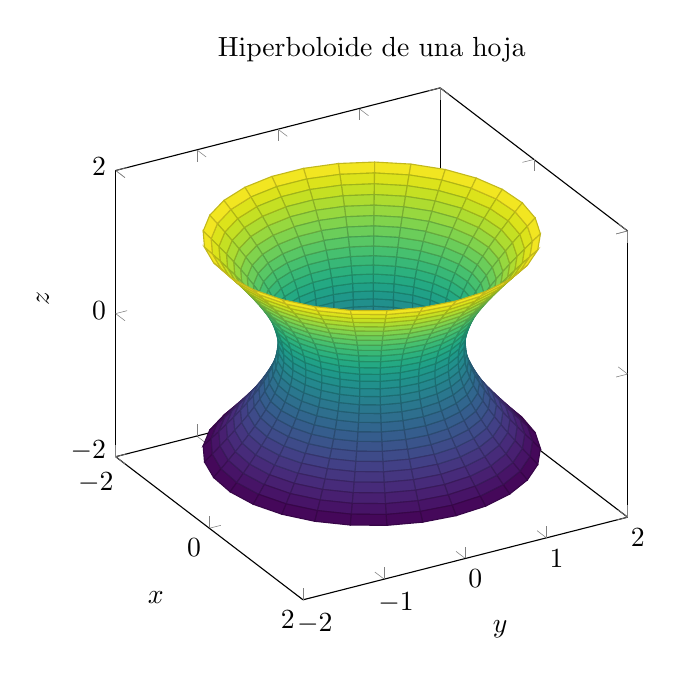
\begin{tikzpicture}
\begin{axis}[
    view={60}{30},
    width=\textwidth/1.5,
    height=\textwidth/1.5,
    xlabel=$x$,
    ylabel=$y$,
    zlabel=$z$,
    z buffer=sort,
    xmin=-2,xmax=2,ymin=-2,ymax=2,zmin=-2,zmax=2,
    title={Hiperboloide de una hoja},
]
\addplot3[
    surf,
    colormap/viridis,
    samples=30,
    samples y=30,
    domain=-1.5:1.5,
    y domain=0:2*pi,
    variable=\z,
    variable y=\theta
]
({sqrt(1+\z^2)*cos(deg(\theta))}, {sqrt(1+\z^2)*sin(deg(\theta))}, {\z});
\end{axis}
\end{tikzpicture}

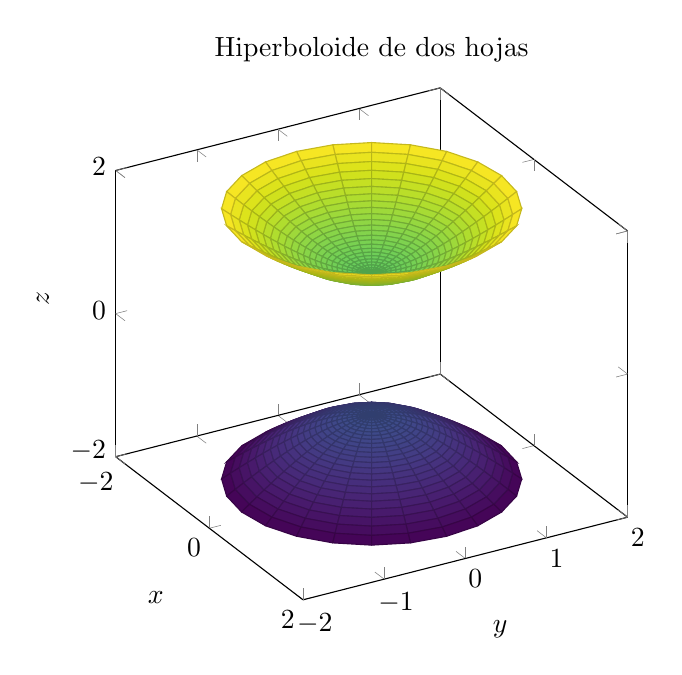
\begin{tikzpicture}
  \begin{axis}[
    unbounded coords=jump,
    view={60}{30},
    width=\textwidth/1.5,
    height=\textwidth/1.5,
    xlabel=$x$,
    ylabel=$y$,
    zlabel=$z$,
    z buffer=sort,
    xmin=-2,xmax=2,ymin=-2,ymax=2,zmin=-2,zmax=2,
    title={Hiperboloide de dos hojas},
]
\addplot3[
    surf,
    unbounded coords=jump,
    colormap/viridis,
    samples=25,
    samples y=25,
    domain=0:1.25,
    y domain=0:2*pi,
    variable=\z,
    variable y=\theta
]
% ({-sqrt(\z^2-1)*cos(deg(\theta))}, {-sqrt(\z^2-1)*sin(deg(\theta))}, {\z});
({sinh(\z)*cos(deg(\theta))}, {sinh(\z)*sin(deg(\theta))}, {cosh(\z)});
\addplot3[
    surf,
    unbounded coords=jump,
    colormap/viridis,
    samples=25,
    samples y=25,
    domain=0:1.25,
    y domain=0:2*pi,
    variable=\z,
    variable y=\theta
]
({sinh(\z)*cos(deg(\theta))}, {sinh(\z)*sin(deg(\theta))}, {-cosh(\z)});
\end{axis}
\end{tikzpicture}

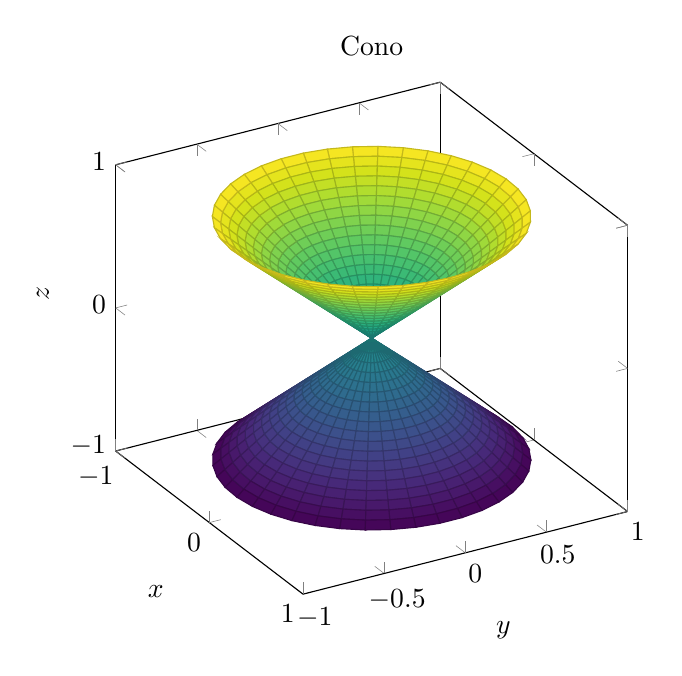
\begin{tikzpicture}
\begin{axis}[
    view={60}{30},
    width=\textwidth/1.5,
    height=\textwidth/1.5,
    xlabel=$x$,
    ylabel=$y$,
    zlabel=$z$,
    z buffer=sort,
    xmin=-1,xmax=1,ymin=-1,ymax=1,zmin=-1,zmax=1,
    title={Cono},
]
\addplot3[
    surf,
    colormap/viridis,
    samples=40,
    samples y=40,
    domain=-0.85:0.85,
    y domain=0:2*pi,
    variable=\z,
    variable y=\theta
]
({\z*cos(deg(\theta))}, {\z*sin(deg(\theta))}, {\z});
\end{axis}
\end{tikzpicture}

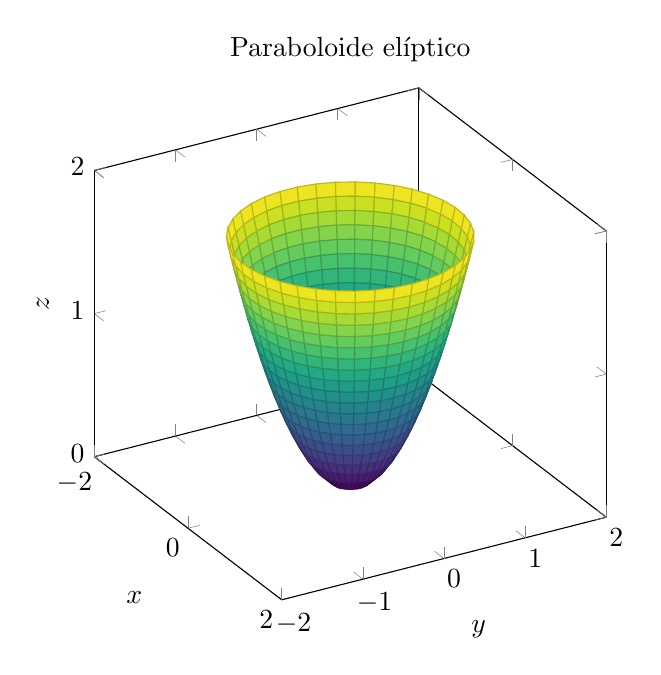
\begin{tikzpicture}
  \begin{axis}[
    unbounded coords=jump,
    view={60}{30},
    width=\textwidth/1.5,
    height=\textwidth/1.5,
    xlabel=$x$,
    ylabel=$y$,
    zlabel=$z$,
    z buffer=sort,
    xmin=-2,xmax=2,ymin=-2,ymax=2,zmin=0,zmax=2,
    title={Paraboloide elíptico},
]
\addplot3[
    surf,
    colormap/viridis,
    samples=40,
    samples y=40,
    domain=-1.75:1.75,
    y domain=0:2*pi,
    variable=\z,
    variable y=\theta
]
({sqrt(\z)*cos(deg(\theta))}, {sqrt(\z)*sin(deg(\theta))}, {\z});
\end{axis}
\end{tikzpicture}

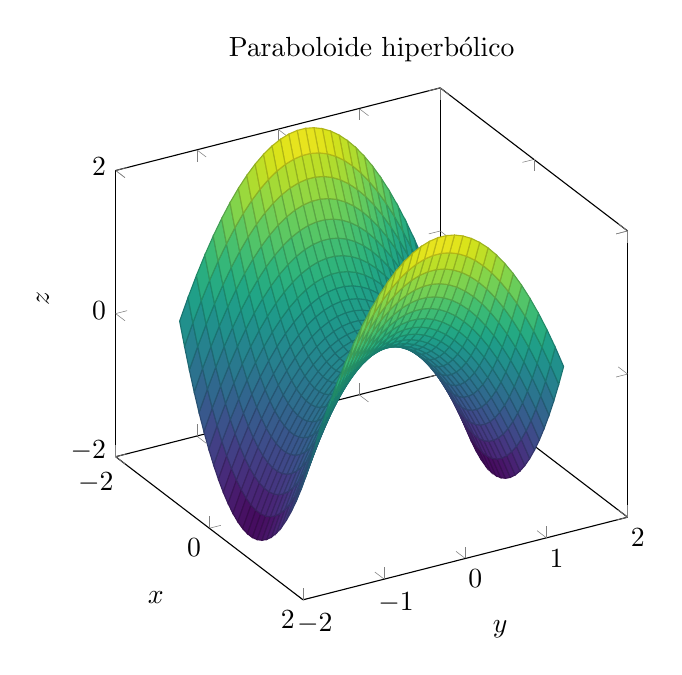
\begin{tikzpicture}
  \begin{axis}[
    unbounded coords=jump,
    view={60}{30},
    width=\textwidth/1.5,
    height=\textwidth/1.5,
    xlabel=$x$,
    ylabel=$y$,
    zlabel=$z$,
    z buffer=sort,
    xmin=-2,xmax=2,ymin=-2,ymax=2,zmin=-2,zmax=2,
    title={Paraboloide hiperbólico},
]
\addplot3[
    surf,
    colormap/viridis,
    samples=30,
    samples y=30,
    domain=-1.5:1.5,
    y domain=-1.5:1.5,
]
{x^2-y^2};
\end{axis}
\end{tikzpicture}

\end{document}
